%----------------------------------------------------------------------------------------
%    PACKAGES AND THEMES
%----------------------------------------------------------------------------------------

\documentclass[aspectratio=169,xcolor=dvipsnames]{beamer}
\usetheme{SimpleDarkBlue}

\usepackage{hyperref}
\usepackage{graphicx} % Allows including images
\usepackage{booktabs} % Allows the use of \toprule, \midrule and \bottomrule in tables
\usepackage{pgfgantt}
\usepackage{tikz}
\usetikzlibrary{shapes.geometric, arrows.meta}

\tikzstyle{startstop} = [rectangle, rounded corners, minimum width=3cm, minimum height=1cm, text centered, draw=black, fill=red!20]
\tikzstyle{process} = [rectangle, minimum width=3cm, minimum height=1cm, text centered, draw=black, fill=orange!20]
\tikzstyle{decision} = [diamond, aspect=2, text centered, draw=black, fill=green!20]
\tikzstyle{arrow} = [thick, ->, >=Stealth]
\tikzstyle{process} = [rectangle, minimum width=3cm, text width=3cm,
                       minimum height=1cm, text centered, draw=black, fill=blue!20]

%----------------------------------------------------------------------------------------
%    TITLE PAGE
%----------------------------------------------------------------------------------------

\title{Evaluating Multimodal Alignment in ChatGPT and
Gemini: An Empirical Study of Inter- and
Intra-Model Consistency in Image Description and
Generation}
%\subtitle{Subtitle}

\author{Saverio Napolitano}

\institute
{
    %Department of Computer Science and Information Engineering \\
    Mid Sweden University % Your institution for the title page
}
\date{\today} % Date, can be changed to a custom date

%----------------------------------------------------------------------------------------
%    PRESENTATION SLIDES
%----------------------------------------------------------------------------------------

\begin{document}

\begin{frame}
    % Print the title page as the first slide
    \titlepage
\end{frame}

\begin{frame}{Overview}
    % Throughout your presentation, if you choose to use \section{} and \subsection{} commands, these will automatically be printed on this slide as an overview of your presentation
    \tableofcontents
\end{frame}

%------------------------------------------------
\section{Problem Statement and Motivation}
%------------------------------------------------

\begin{frame}{Problem Statement and Motivation}
    \begin{itemize}
        \item Intra-AI model: same AI model for both image description and generation
        \item Inter-AI model: different AI models for image description and generation
        \item Important for: trustworthiness, reproducibility, usability in creative, scientific and industrial contexts
        \item Research gap: lack of comprehensive analysis comparing intra-AI model and inter-AI model alignment in image description and generation tasks, combining human and automatic evaluation.
    \end{itemize}
\end{frame}

%------------------------------------------------
\section{Research Questions}
%------------------------------------------------

\begin{frame}{Research Questions}
    \begin{enumerate}
        \item \emph{How consistent, with respect to human preferences, are multimodal AI models in aligning descrip-
tions and generations, both within the same model and across different models?}
        \item \emph{How well do automatic multimodal evaluation metrics align with human judgments?} 
    \end{enumerate}
\end{frame}

%------------------------------------------------
\section{Related Work}
%------------------------------------------------

\begin{frame}{Related Work}
    \begin{itemize}
        \item CLIP-AGIQA \cite{tang2024clipagiqa}
        \begin{itemize}
            \item Automatic evaluation metric for image generation quality and alignment
        \end{itemize}
    \end{itemize}
    \begin{figure} 
        \centering
        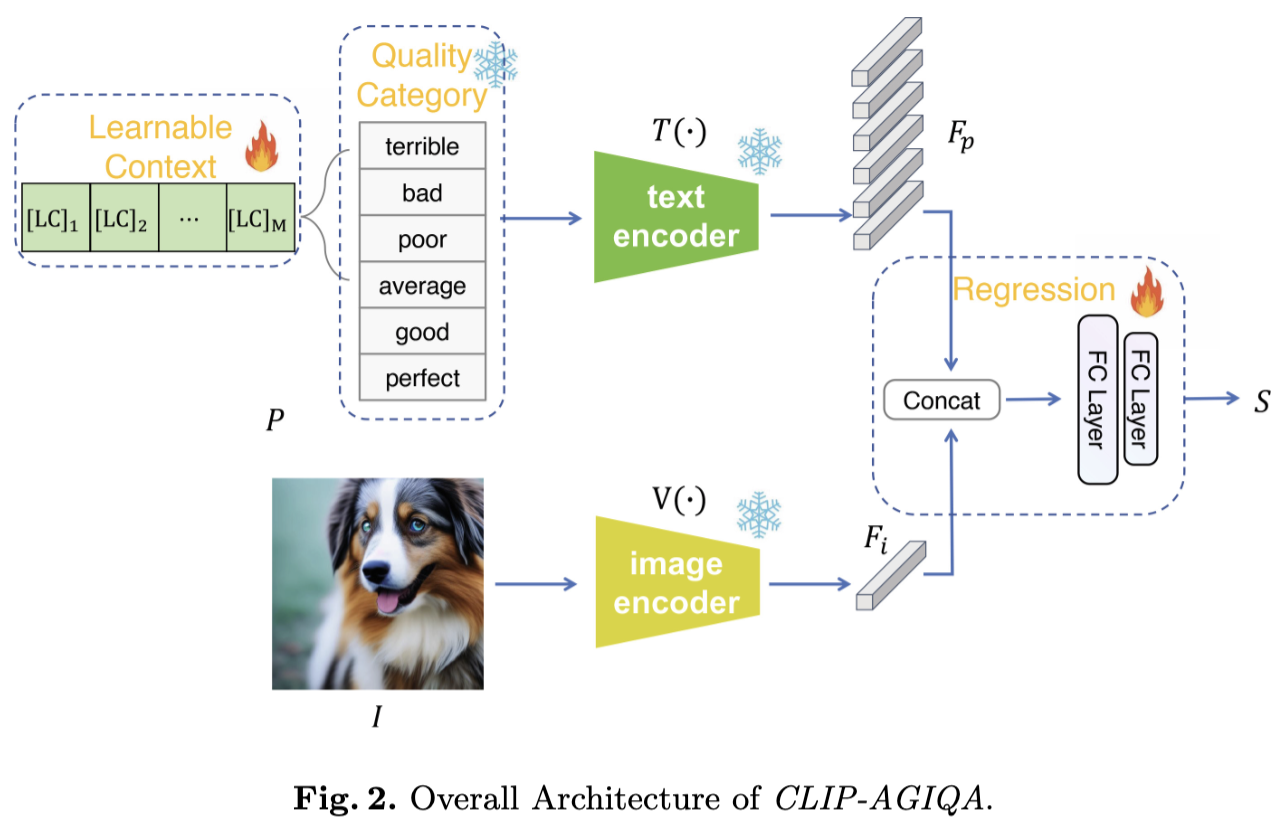
\includegraphics[height=0.75\textheight]{figures/clip_agiqa.png}
        \label{fig:Fig. 2}
    \end{figure}
\end{frame}

%------------------------------------------------
\section{Research Method}
%------------------------------------------------

\begin{frame}{Research Method}
    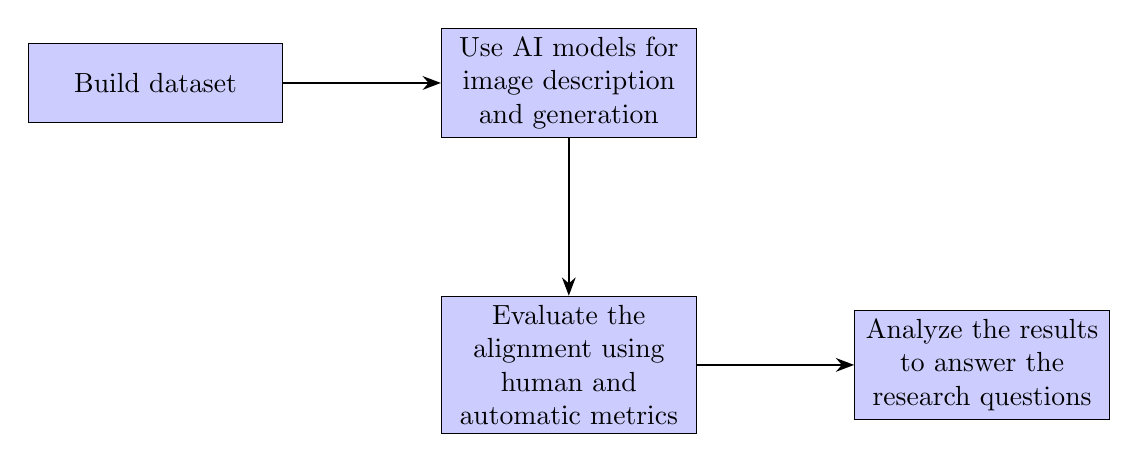
\begin{tikzpicture}[node distance=2cm]

        \node (p1) [process] {Build dataset};
        \node (p2) [process, right=of p1] {Use AI models for image description and generation};
        \node (p3) [process, below=of p2] {Evaluate the alignment using human and automatic metrics};
        \node (p4) [process, right=of p3] {Analyze the results to answer the research questions};

        \draw [arrow] (p1) -- (p2);
        \draw [arrow] (p2) -- (p3);
        \draw [arrow] (p3) -- (p4);

    \end{tikzpicture}
\end{frame}

%------------------------------------------------
\subsection{Dataset}
%------------------------------------------------

\begin{frame}{Dataset}
    \begin{itemize}
        \item 10--15 images
        \item Collected explicitly for this study
        \item Objects, nature, people, text
    \end{itemize}
\end{frame}

%------------------------------------------------
\subsection{Prompts}
%------------------------------------------------

\begin{frame}{Prompts}
    \begin{itemize}
        \item Basic task description 
        \item Detailed task description, specifying target audience
        \item Detailed task description, specifying target audience and their purpose
    \end{itemize}
\end{frame}

%------------------------------------------------
\subsection{Evaluation Criteria}
%------------------------------------------------

\begin{frame}{Evaluation Criteria}
    \begin{itemize}
        \item Automatic metrics
        \begin{itemize}
            \item CLIP-AGIQA
        \end{itemize}
        \item Human judgments
        \begin{itemize}
            \item 5--10 evaluators
            \item Ranking output images based on provided reference 
        \end{itemize}
    \end{itemize}
\end{frame}

%------------------------------------------------
\subsection{Results Analysis}
%------------------------------------------------

\begin{frame}{Results Analysis}
    \begin{itemize}
        \item Inter-rater agreement
        \begin{itemize}
            \item Kendall's W
        \end{itemize}
        \item Correlation between human ranking and automatic metrics
        \begin{itemize}
            \item Kendall's Tau
            \item Spearman correlation 
        \end{itemize}
    \end{itemize}
\end{frame}

%------------------------------------------------
\section{Expected Results}
%------------------------------------------------

\begin{frame}{Expected Results}
    \begin{enumerate}
        \item \emph{Inter-AI model alignment will show significant divergence due to architectural heterogeneity, while
intra-AI model descriptive vs. generative outputs will diverge less but still systematically} 
        \item \emph{CLIP-based automatic metrics will partially but not fully capture human preferences, requiring
complementary human evaluation}
    \end{enumerate}
\end{frame}

%------------------------------------------------
\section{Time Plan}
%------------------------------------------------

\begin{frame}{Time Plan}
    \centering
    \begin{ganttchart}[
        time slot format=isodate,      % daily input
        x unit=0.11cm,                 % << adjust this to change width
        hgrid,
        vgrid,
        y unit title=0.5cm,
        y unit chart=0.6cm,
        title label font=\scriptsize\bfseries,
        title height=1,
        bar label font=\scriptsize,
        group label font=\scriptsize
    ]{2025-10-13}{2026-01-11}

    % 13 ISO weeks from 2025-10-13 to 2026-01-11:
    % 42,43,...,52,1,2
    \gantttitlelist{42,43,44,45,46,47,48,49,50,51,52,1,2}{7} \\

    \ganttbar{Proposal Review}{2025-10-13}{2025-10-19} \\
    \ganttbar{Dataset Preparation}{2025-10-20}{2025-11-02} \\
    \ganttbar{Model Experiments}{2025-11-03}{2025-11-16} \\
    \ganttbar{Evaluation (Auto + Human)}{2025-11-16}{2025-11-30} \\
    \ganttbar{Results Analysis}{2025-12-01}{2025-12-07} \\
    \ganttbar{Article Writing}{2025-11-03}{2025-12-13} \\
    \ganttbar{Peer Review}{2025-12-14}{2025-12-21} \\
    \ganttbar{Project Presentation}{2025-12-22}{2026-01-11}

    \end{ganttchart}
\end{frame}

\begin{frame}{References}
    \footnotesize
    \bibliography{references.bib}
    \bibliographystyle{apalike}
\end{frame}

\begin{frame}
    \Huge{\centerline{\textbf{Thank You}}}
\end{frame}

%----------------------------------------------------------------------------------------

\end{document}